% Created by tikzDevice version 0.10.1 on 2016-09-01 14:08:23
% !TEX encoding = UTF-8 Unicode
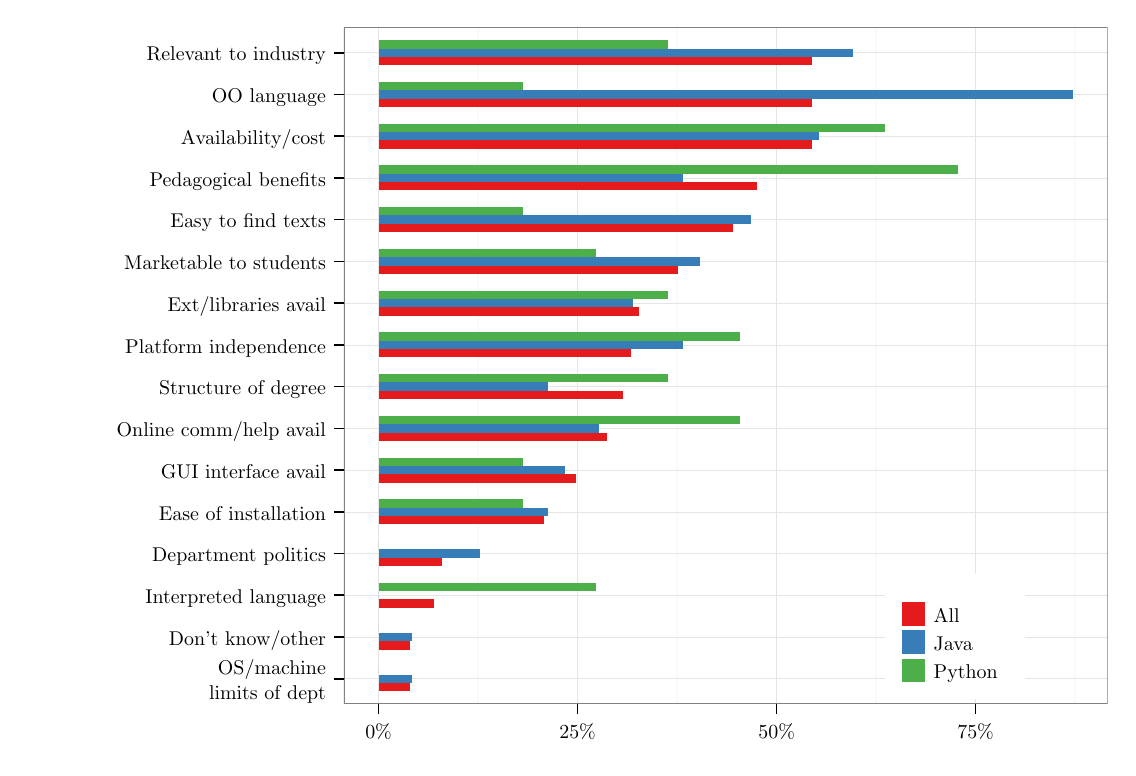
\begin{tikzpicture}[x=1.2pt,y=1.2pt]
\definecolor{fillColor}{RGB}{255,255,255}
\path[use as bounding box,fill=fillColor,fill opacity=0.00] (0,0) rectangle (325.21,216.81);
\begin{scope}
\path[clip] (  0.00,  0.00) rectangle (325.21,216.81);
\definecolor{drawColor}{RGB}{255,255,255}
\definecolor{fillColor}{RGB}{255,255,255}

\path[draw=drawColor,line width= 0.6pt,line join=round,line cap=round,fill=fillColor] (  0.00,  0.00) rectangle (325.21,216.81);
\end{scope}
\begin{scope}
\path[clip] ( 95.21, 13.20) rectangle (325.21,216.81);
\definecolor{fillColor}{RGB}{255,255,255}

\path[fill=fillColor] ( 95.21, 13.20) rectangle (325.21,216.81);
\definecolor{drawColor}{gray}{0.98}

\path[draw=drawColor,line width= 0.6pt,line join=round] (135.63, 13.20) --
	(135.63,216.81);

\path[draw=drawColor,line width= 0.6pt,line join=round] (195.55, 13.20) --
	(195.55,216.81);

\path[draw=drawColor,line width= 0.6pt,line join=round] (255.48, 13.20) --
	(255.48,216.81);

\path[draw=drawColor,line width= 0.6pt,line join=round] (315.41, 13.20) --
	(315.41,216.81);
\definecolor{drawColor}{gray}{0.90}

\path[draw=drawColor,line width= 0.2pt,line join=round] ( 95.21, 20.75) --
	(325.21, 20.75);

\path[draw=drawColor,line width= 0.2pt,line join=round] ( 95.21, 33.31) --
	(325.21, 33.31);

\path[draw=drawColor,line width= 0.2pt,line join=round] ( 95.21, 45.88) --
	(325.21, 45.88);

\path[draw=drawColor,line width= 0.2pt,line join=round] ( 95.21, 58.45) --
	(325.21, 58.45);

\path[draw=drawColor,line width= 0.2pt,line join=round] ( 95.21, 71.02) --
	(325.21, 71.02);

\path[draw=drawColor,line width= 0.2pt,line join=round] ( 95.21, 83.59) --
	(325.21, 83.59);

\path[draw=drawColor,line width= 0.2pt,line join=round] ( 95.21, 96.15) --
	(325.21, 96.15);

\path[draw=drawColor,line width= 0.2pt,line join=round] ( 95.21,108.72) --
	(325.21,108.72);

\path[draw=drawColor,line width= 0.2pt,line join=round] ( 95.21,121.29) --
	(325.21,121.29);

\path[draw=drawColor,line width= 0.2pt,line join=round] ( 95.21,133.86) --
	(325.21,133.86);

\path[draw=drawColor,line width= 0.2pt,line join=round] ( 95.21,146.43) --
	(325.21,146.43);

\path[draw=drawColor,line width= 0.2pt,line join=round] ( 95.21,159.00) --
	(325.21,159.00);

\path[draw=drawColor,line width= 0.2pt,line join=round] ( 95.21,171.56) --
	(325.21,171.56);

\path[draw=drawColor,line width= 0.2pt,line join=round] ( 95.21,184.13) --
	(325.21,184.13);

\path[draw=drawColor,line width= 0.2pt,line join=round] ( 95.21,196.70) --
	(325.21,196.70);

\path[draw=drawColor,line width= 0.2pt,line join=round] ( 95.21,209.27) --
	(325.21,209.27);

\path[draw=drawColor,line width= 0.2pt,line join=round] (105.66, 13.20) --
	(105.66,216.81);

\path[draw=drawColor,line width= 0.2pt,line join=round] (165.59, 13.20) --
	(165.59,216.81);

\path[draw=drawColor,line width= 0.2pt,line join=round] (225.52, 13.20) --
	(225.52,216.81);

\path[draw=drawColor,line width= 0.2pt,line join=round] (285.44, 13.20) --
	(285.44,216.81);
\definecolor{fillColor}{RGB}{228,26,28}

\path[fill=fillColor] (105.66, 16.97) rectangle (115.16, 19.49);
\definecolor{fillColor}{RGB}{55,126,184}

\path[fill=fillColor] (105.66, 19.49) rectangle (115.87, 22.00);
\definecolor{fillColor}{RGB}{77,175,74}

\path[fill=fillColor] (105.66, 22.00) rectangle (105.66, 24.52);
\definecolor{fillColor}{RGB}{228,26,28}

\path[fill=fillColor] (105.66, 29.54) rectangle (115.16, 32.06);
\definecolor{fillColor}{RGB}{55,126,184}

\path[fill=fillColor] (105.66, 32.06) rectangle (115.87, 34.57);
\definecolor{fillColor}{RGB}{77,175,74}

\path[fill=fillColor] (105.66, 34.57) rectangle (105.66, 37.08);
\definecolor{fillColor}{RGB}{228,26,28}

\path[fill=fillColor] (105.66, 42.11) rectangle (122.27, 44.62);
\definecolor{fillColor}{RGB}{55,126,184}

\path[fill=fillColor] (105.66, 44.62) rectangle (105.66, 47.14);
\definecolor{fillColor}{RGB}{77,175,74}

\path[fill=fillColor] (105.66, 47.14) rectangle (171.03, 49.65);
\definecolor{fillColor}{RGB}{228,26,28}

\path[fill=fillColor] (105.66, 54.68) rectangle (124.65, 57.19);
\definecolor{fillColor}{RGB}{55,126,184}

\path[fill=fillColor] (105.66, 57.19) rectangle (136.27, 59.71);
\definecolor{fillColor}{RGB}{77,175,74}

\path[fill=fillColor] (105.66, 59.71) rectangle (105.66, 62.22);
\definecolor{fillColor}{RGB}{228,26,28}

\path[fill=fillColor] (105.66, 67.25) rectangle (155.50, 69.76);
\definecolor{fillColor}{RGB}{55,126,184}

\path[fill=fillColor] (105.66, 69.76) rectangle (156.67, 72.27);
\definecolor{fillColor}{RGB}{77,175,74}

\path[fill=fillColor] (105.66, 72.27) rectangle (149.24, 74.79);
\definecolor{fillColor}{RGB}{228,26,28}

\path[fill=fillColor] (105.66, 79.82) rectangle (164.99, 82.33);
\definecolor{fillColor}{RGB}{55,126,184}

\path[fill=fillColor] (105.66, 82.33) rectangle (161.75, 84.84);
\definecolor{fillColor}{RGB}{77,175,74}

\path[fill=fillColor] (105.66, 84.84) rectangle (149.24, 87.36);
\definecolor{fillColor}{RGB}{228,26,28}

\path[fill=fillColor] (105.66, 92.38) rectangle (174.48, 94.90);
\definecolor{fillColor}{RGB}{55,126,184}

\path[fill=fillColor] (105.66, 94.90) rectangle (171.97, 97.41);
\definecolor{fillColor}{RGB}{77,175,74}

\path[fill=fillColor] (105.66, 97.41) rectangle (214.61, 99.93);
\definecolor{fillColor}{RGB}{228,26,28}

\path[fill=fillColor] (105.66,104.95) rectangle (179.23,107.47);
\definecolor{fillColor}{RGB}{55,126,184}

\path[fill=fillColor] (105.66,107.47) rectangle (156.67,109.98);
\definecolor{fillColor}{RGB}{77,175,74}

\path[fill=fillColor] (105.66,109.98) rectangle (192.82,112.49);
\definecolor{fillColor}{RGB}{228,26,28}

\path[fill=fillColor] (105.66,117.52) rectangle (181.60,120.03);
\definecolor{fillColor}{RGB}{55,126,184}

\path[fill=fillColor] (105.66,120.03) rectangle (197.47,122.55);
\definecolor{fillColor}{RGB}{77,175,74}

\path[fill=fillColor] (105.66,122.55) rectangle (214.61,125.06);
\definecolor{fillColor}{RGB}{228,26,28}

\path[fill=fillColor] (105.66,130.09) rectangle (183.98,132.60);
\definecolor{fillColor}{RGB}{55,126,184}

\path[fill=fillColor] (105.66,132.60) rectangle (182.15,135.12);
\definecolor{fillColor}{RGB}{77,175,74}

\path[fill=fillColor] (105.66,135.12) rectangle (192.82,137.63);
\definecolor{fillColor}{RGB}{228,26,28}

\path[fill=fillColor] (105.66,142.66) rectangle (195.84,145.17);
\definecolor{fillColor}{RGB}{55,126,184}

\path[fill=fillColor] (105.66,145.17) rectangle (202.58,147.68);
\definecolor{fillColor}{RGB}{77,175,74}

\path[fill=fillColor] (105.66,147.68) rectangle (171.03,150.20);
\definecolor{fillColor}{RGB}{228,26,28}

\path[fill=fillColor] (105.66,155.23) rectangle (212.45,157.74);
\definecolor{fillColor}{RGB}{55,126,184}

\path[fill=fillColor] (105.66,157.74) rectangle (217.87,160.25);
\definecolor{fillColor}{RGB}{77,175,74}

\path[fill=fillColor] (105.66,160.25) rectangle (149.24,162.77);
\definecolor{fillColor}{RGB}{228,26,28}

\path[fill=fillColor] (105.66,167.79) rectangle (219.57,170.31);
\definecolor{fillColor}{RGB}{55,126,184}

\path[fill=fillColor] (105.66,170.31) rectangle (197.47,172.82);
\definecolor{fillColor}{RGB}{77,175,74}

\path[fill=fillColor] (105.66,172.82) rectangle (280.00,175.33);
\definecolor{fillColor}{RGB}{228,26,28}

\path[fill=fillColor] (105.66,180.36) rectangle (236.21,182.88);
\definecolor{fillColor}{RGB}{55,126,184}

\path[fill=fillColor] (105.66,182.88) rectangle (238.27,185.39);
\definecolor{fillColor}{RGB}{77,175,74}

\path[fill=fillColor] (105.66,185.39) rectangle (258.21,187.90);
\definecolor{fillColor}{RGB}{228,26,28}

\path[fill=fillColor] (105.66,192.93) rectangle (236.21,195.44);
\definecolor{fillColor}{RGB}{55,126,184}

\path[fill=fillColor] (105.66,195.44) rectangle (314.76,197.96);
\definecolor{fillColor}{RGB}{77,175,74}

\path[fill=fillColor] (105.66,197.96) rectangle (149.24,200.47);
\definecolor{fillColor}{RGB}{228,26,28}

\path[fill=fillColor] (105.66,205.50) rectangle (236.21,208.01);
\definecolor{fillColor}{RGB}{55,126,184}

\path[fill=fillColor] (105.66,208.01) rectangle (248.46,210.53);
\definecolor{fillColor}{RGB}{77,175,74}

\path[fill=fillColor] (105.66,210.53) rectangle (192.82,213.04);
\definecolor{drawColor}{gray}{0.50}

\path[draw=drawColor,line width= 0.6pt,line join=round,line cap=round] ( 95.21, 13.20) rectangle (325.21,216.81);
\end{scope}
\begin{scope}
\path[clip] (  0.00,  0.00) rectangle (325.21,216.81);
\definecolor{drawColor}{RGB}{0,0,0}

\node[text=drawColor,anchor=base east,inner sep=0pt, outer sep=0pt, scale=  0.72] at ( 89.81, 22.15) {OS/machine};

\node[text=drawColor,anchor=base east,inner sep=0pt, outer sep=0pt, scale=  0.72] at ( 89.81, 14.38) {limits of dept};

\node[text=drawColor,anchor=base east,inner sep=0pt, outer sep=0pt, scale=  0.72] at ( 89.81, 30.83) {Don't know/other};

\node[text=drawColor,anchor=base east,inner sep=0pt, outer sep=0pt, scale=  0.72] at ( 89.81, 43.40) {Interpreted language};

\node[text=drawColor,anchor=base east,inner sep=0pt, outer sep=0pt, scale=  0.72] at ( 89.81, 55.97) {Department politics};

\node[text=drawColor,anchor=base east,inner sep=0pt, outer sep=0pt, scale=  0.72] at ( 89.81, 68.54) {Ease of installation};

\node[text=drawColor,anchor=base east,inner sep=0pt, outer sep=0pt, scale=  0.72] at ( 89.81, 81.11) {GUI interface avail};

\node[text=drawColor,anchor=base east,inner sep=0pt, outer sep=0pt, scale=  0.72] at ( 89.81, 93.68) {Online comm/help avail};

\node[text=drawColor,anchor=base east,inner sep=0pt, outer sep=0pt, scale=  0.72] at ( 89.81,106.24) {Structure of degree};

\node[text=drawColor,anchor=base east,inner sep=0pt, outer sep=0pt, scale=  0.72] at ( 89.81,118.81) {Platform independence};

\node[text=drawColor,anchor=base east,inner sep=0pt, outer sep=0pt, scale=  0.72] at ( 89.81,131.38) {Ext/libraries avail};

\node[text=drawColor,anchor=base east,inner sep=0pt, outer sep=0pt, scale=  0.72] at ( 89.81,143.95) {Marketable to students};

\node[text=drawColor,anchor=base east,inner sep=0pt, outer sep=0pt, scale=  0.72] at ( 89.81,156.52) {Easy to find texts};

\node[text=drawColor,anchor=base east,inner sep=0pt, outer sep=0pt, scale=  0.72] at ( 89.81,169.08) {Pedagogical benefits};

\node[text=drawColor,anchor=base east,inner sep=0pt, outer sep=0pt, scale=  0.72] at ( 89.81,181.65) {Availability/cost};

\node[text=drawColor,anchor=base east,inner sep=0pt, outer sep=0pt, scale=  0.72] at ( 89.81,194.22) {OO language};

\node[text=drawColor,anchor=base east,inner sep=0pt, outer sep=0pt, scale=  0.72] at ( 89.81,206.79) {Relevant to industry};
\end{scope}
\begin{scope}
\path[clip] (  0.00,  0.00) rectangle (325.21,216.81);
\definecolor{drawColor}{RGB}{0,0,0}

\path[draw=drawColor,line width= 0.6pt,line join=round] ( 92.21, 20.75) --
	( 95.21, 20.75);

\path[draw=drawColor,line width= 0.6pt,line join=round] ( 92.21, 33.31) --
	( 95.21, 33.31);

\path[draw=drawColor,line width= 0.6pt,line join=round] ( 92.21, 45.88) --
	( 95.21, 45.88);

\path[draw=drawColor,line width= 0.6pt,line join=round] ( 92.21, 58.45) --
	( 95.21, 58.45);

\path[draw=drawColor,line width= 0.6pt,line join=round] ( 92.21, 71.02) --
	( 95.21, 71.02);

\path[draw=drawColor,line width= 0.6pt,line join=round] ( 92.21, 83.59) --
	( 95.21, 83.59);

\path[draw=drawColor,line width= 0.6pt,line join=round] ( 92.21, 96.15) --
	( 95.21, 96.15);

\path[draw=drawColor,line width= 0.6pt,line join=round] ( 92.21,108.72) --
	( 95.21,108.72);

\path[draw=drawColor,line width= 0.6pt,line join=round] ( 92.21,121.29) --
	( 95.21,121.29);

\path[draw=drawColor,line width= 0.6pt,line join=round] ( 92.21,133.86) --
	( 95.21,133.86);

\path[draw=drawColor,line width= 0.6pt,line join=round] ( 92.21,146.43) --
	( 95.21,146.43);

\path[draw=drawColor,line width= 0.6pt,line join=round] ( 92.21,159.00) --
	( 95.21,159.00);

\path[draw=drawColor,line width= 0.6pt,line join=round] ( 92.21,171.56) --
	( 95.21,171.56);

\path[draw=drawColor,line width= 0.6pt,line join=round] ( 92.21,184.13) --
	( 95.21,184.13);

\path[draw=drawColor,line width= 0.6pt,line join=round] ( 92.21,196.70) --
	( 95.21,196.70);

\path[draw=drawColor,line width= 0.6pt,line join=round] ( 92.21,209.27) --
	( 95.21,209.27);
\end{scope}
\begin{scope}
\path[clip] (  0.00,  0.00) rectangle (325.21,216.81);
\definecolor{drawColor}{RGB}{0,0,0}

\path[draw=drawColor,line width= 0.6pt,line join=round] (105.66, 10.20) --
	(105.66, 13.20);

\path[draw=drawColor,line width= 0.6pt,line join=round] (165.59, 10.20) --
	(165.59, 13.20);

\path[draw=drawColor,line width= 0.6pt,line join=round] (225.52, 10.20) --
	(225.52, 13.20);

\path[draw=drawColor,line width= 0.6pt,line join=round] (285.44, 10.20) --
	(285.44, 13.20);
\end{scope}
\begin{scope}
\path[clip] (  0.00,  0.00) rectangle (325.21,216.81);
\definecolor{drawColor}{RGB}{0,0,0}

\node[text=drawColor,anchor=base,inner sep=0pt, outer sep=0pt, scale=  0.72] at (105.66,  2.85) {0\%};

\node[text=drawColor,anchor=base,inner sep=0pt, outer sep=0pt, scale=  0.72] at (165.59,  2.85) {25\%};

\node[text=drawColor,anchor=base,inner sep=0pt, outer sep=0pt, scale=  0.72] at (225.52,  2.85) {50\%};

\node[text=drawColor,anchor=base,inner sep=0pt, outer sep=0pt, scale=  0.72] at (285.44,  2.85) {75\%};
\end{scope}
\begin{scope}
\path[clip] (  0.00,  0.00) rectangle (325.21,216.81);
\definecolor{fillColor}{RGB}{255,255,255}

\path[fill=fillColor] (258.23, 14.69) rectangle (300.20, 52.44);
\end{scope}
\begin{scope}
\path[clip] (  0.00,  0.00) rectangle (325.21,216.81);
\definecolor{fillColor}{RGB}{228,26,28}

\path[fill=fillColor] (263.21, 36.74) rectangle (270.32, 43.85);
\end{scope}
\begin{scope}
\path[clip] (  0.00,  0.00) rectangle (325.21,216.81);
\definecolor{fillColor}{RGB}{55,126,184}

\path[fill=fillColor] (263.21, 28.20) rectangle (270.32, 35.31);
\end{scope}
\begin{scope}
\path[clip] (  0.00,  0.00) rectangle (325.21,216.81);
\definecolor{fillColor}{RGB}{77,175,74}

\path[fill=fillColor] (263.21, 19.67) rectangle (270.32, 26.78);
\end{scope}
\begin{scope}
\path[clip] (  0.00,  0.00) rectangle (325.21,216.81);
\definecolor{drawColor}{RGB}{0,0,0}

\node[text=drawColor,anchor=base west,inner sep=0pt, outer sep=0pt, scale=  0.72] at (272.84, 37.81) {All};
\end{scope}
\begin{scope}
\path[clip] (  0.00,  0.00) rectangle (325.21,216.81);
\definecolor{drawColor}{RGB}{0,0,0}

\node[text=drawColor,anchor=base west,inner sep=0pt, outer sep=0pt, scale=  0.72] at (272.84, 29.28) {Java};
\end{scope}
\begin{scope}
\path[clip] (  0.00,  0.00) rectangle (325.21,216.81);
\definecolor{drawColor}{RGB}{0,0,0}

\node[text=drawColor,anchor=base west,inner sep=0pt, outer sep=0pt, scale=  0.72] at (272.84, 20.74) {Python};
\end{scope}
\end{tikzpicture}
